\chapter{Conclusion}

This chapter briefly summarises the approach of this thesis, and then goes on to sum up the key findings from the field works. Finally, the thesis concludes with limitations and an outlook on future work that this thesis might inspire.\\

\section{Summary of approach}
This PhD work use Mixed reality game - AtomicOrchid as a testbeds to probe the design implications for agent planning support system. Field trials were conducted for the three versions of AtomicOrchid game with different interaction design patterns. The first one is a non agent version of the game. The second and third studies are planned to probe two interaction design patterns (HuOL and HuIL). Video and system logs of the field trails has been collected and interaction analysis has been conducted to generate requirements and interaction design implications. \\


\section{Summary of findings}
Three studies are carried out iteratively. The AtomicOrchid system evolves throughout the three studies. The interaction design for the study 2 and 3 follows the design patterns (HuOL and HuIL), but are also inspired by key observations from previous studies. The key observations constitute important part of the contributions of the PhD work. In what follows, the section will go through the key observations and how they influence system evolution across the 3 field trials \\ 

\begin{figure}[h]
  \centering
  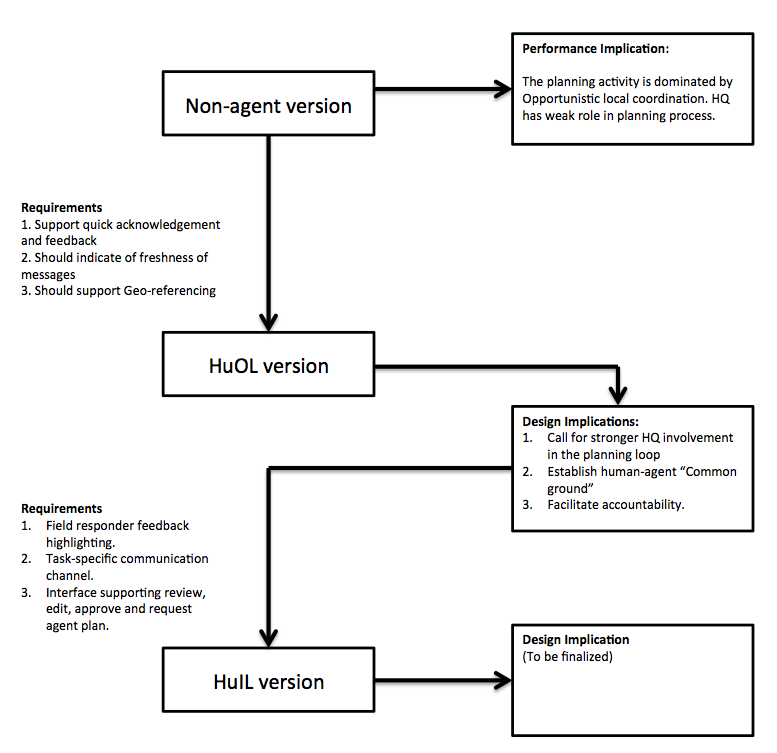
\includegraphics[width=1\textwidth]{img/conclusion/connections}
  \caption{Requirments and Implications generated from each study}
  \label{fig:connections}
\end{figure}

The non-agent AtomicOrchid trial (study 1) is aimed to establish baseline performance of human planning in the time and spatially constrained disaster settings and to generate general requirements of coordination support system which is also applicable to the next two agent-integrated version of AtomicOrchid. The result of interaction analysis showed that the HQ players who are supposed to perform planning for the whole team has little influence on the actual planning activities. The observation showed that team planning is dominated by local coordination between field players with opportunistic manner. The findings confirms the opportunity for agent planning support which may be able generate quicker and optimised plan for the player team. Apart from observations on team performance, several general requirements for coordination systems are generated (see figure \ref{fig:connections}).\\

In study 2, a planning agent is integrated to the system with the HuOL interaction design. The general requirements from study 1 leads to a number of system improvements(see figure \ref{fig:connections}) in study 2, which help us to avoid non-agent related factors in field trials. Through interaction analysis, we find division of labour between human and agent (see section \ref{sec:studytwointroduction}) in which the agent takes over routine planning activities while the human focus on other issues such as navigation. However, there are also evidence showing the agent planning occasionally interrupts workflow of human team because it fails to consider social cost and coordination overhead of task changes. We also observed HQ player struggled to influence the plan because the lack of interface level support. Further, a set of misconceptions in feedback loops (see section \ref{sec:studytwofeedback}) are also observed.\\

In study 3, the system is evolved to facilitate HuIL interaction with the feedback from study 2. The main changes are a number of interface functionalities which enable HQ to approve, edit agent planning and monitor player feedbacks. Through observing the usage of this new functionalities in the control room, we found a new pattern division of labour between in which:
	\begin{enumerate}
	 \item The HQ decide when to perform re-plan.
	 \item The HQ review every agent instruction for routine task planning.
	 \item The planning agent deals with player feedback.
	 \item The Agent propose task allocation
	\end{enumerate}
	
Further observation shows that coordination overhead caused by the agent planning (observed in study 2) may have been reduced as a result of greater HQ involvement in the planning. Analysis of some failed cases of coordination also points out a number of issues, which leads to several design implications[ TO be finalised ]  \\


\subsection{HuOL vs HuIL}
The HuOL and HuIL interaction designs have been trialled in two studies. The section will reflect on some of the findings related to the two interaction design patterns. \\

To recap, the main distinction between the two interaction design is the extent to which the human HQ is involved in routine task planning. The HuOL  argues the minimal involvement of human HQ, leaving the agent to deal with the planning. HQ only need to deal with occasional contingencies. The HuIL requires constant HQ agent interaction to ensure the planning quality. Guided by the two patterns, detailed design has been implemented to \\

\begin{figure}[h]
  \centering
  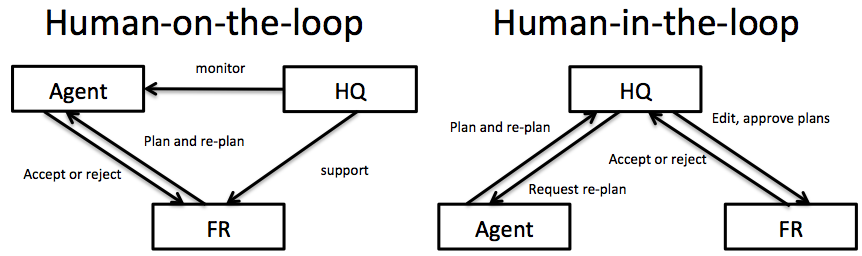
\includegraphics[width=1\textwidth]{img/conclusion/huilvshuol}
  \caption{HuIL vs HuOL}
  \label{fig:huilvshuol}
\end{figure}


There are several performance differences between the HuIL and HuOL studies. Direct comparison of performance between HuIL and HuOL is not applicable because the study 2 introduces a number of interface support (see figure \ref{fig:huilvshuol}) that influences performance as well. However, the difference of performance can still leads to some implications of interaction design.\\

\begin{enumerate}
\item Less coordination overhead in HuIL \\
As we have summarised in section \ref{sec:huilimperfection}, there are evidence showing that the HuOL design is more likely to cause extra coordination overhead when compared to the HuIL design. In study 2, HQ has been observed to deliberately avoid unnecessary task interruptions and team reformations caused by agent planning, which in turn, reduce the coordination overhead. It can be argued that the difference is simply caused by lack of reliability of the agent. Advanced agent planner which can better model the social process involved in task changes and take into account the possible overhead. However, given the social process might be hard to be modelled, the HuIL design can be useful to overcome the agent's limitation and utilise its capability at the same time.\\


\item HQ with a HuIL design maintains higher situational awareness[Need expand in study chapter]\\
As HQ is responsible for review and approval in HuIL design, they are found to maintain higher situational awareness when compared to the HuOL design. The observation is consistent with a well observed phenomena that the Human operator controlling a highly automated system is likely to loss situational awareness.\\


\item HQ's ability to intervene agent planning is stronger in the HuIL study.\\
This performance difference can not be directly linked to the distinction between HuOL and HuIL. In HuOL study, HQ is observed to struggle to influence the planning process, because the only way to intervene the planning is to send unstructured text messages in broadcast channel. HQ's ability to intervene has been greatly enhanced by a set of interface support introduced in the HuIL study. Some of the interface support is inspired by the implications from HuOL study. It highlights the need of interface support for HQ intervention because both HuOL and HuIL requires HQ get involved when necessary. \\

\end{enumerate}

To sum up, the reliability of agent could be one factor when considering interaction design[]. The improvement of reliability can reduce required human involvement, thus, allowing the HuOL design. However, in this PhD study, we assume human behaviour and disaster environment can be hard to be perfectly modelled. Therefore, HuIL design can be employed to overcome the (limited) reliability of the agent.Secondly, situational awareness of HQ can be important for both HuIL and HuOL design, though the study shows HuIL design help HQ to maintain situational awareness. Further, the interface support for HQ intervention has been proved to important in both HuIL and HuOL settings.\\


\subsection{Establishing Common Ground}
Establishing a common ground between human and agent has emerged as a common topic in discussions of both study 2 and study 3. The section will summaries the implications on establishing "Common Ground" from the two agent studies. \\

The "common ground" could be improved from 2 aspects:  1) Appropriate interaction design which allow human operators to understand the agent. 2) technical advancement in terms of algorithm and modelling techniques which enable agents to model human behaviours and process human feedbacks (e.g. agent being able to consider social cost of team reformation). The latter concerns about technical aspect of agent design which is beyond the scope of this PhD work. Therefore, this section will focus on building "Common ground" from the the perspective of interaction design. \\

In both study 2 and 3, the agent behaves like a "black box" which gives the results (task allocation). The interface only exposes the results of agent for HQ to monitoring. Through our observations in chapter \ref{ch:studytwo}, \ref{ch:studythree}, we find there could be some extra information shared between human and agent to improve planning.\\

The HQ players is found (section x.x.x) to occasionally make some forward planning for field players. Because the forward planning is also performed by the agent to derive current plan, the information could be shared so that the HQ players can be provided with the agent suggestion when doing forward planning.\\

The reasoning behind current task allocation would also be useful for sharing. In chapter \ref{ch:studythree} , HQ is found overriding agent plans, which leads to undesirable results. The HQ is also found being confused when agent stop assigning tasks to players with low health. Exposing internal reasoning of the agent can help the HQ to make informed decisions. \\

Misunderstanding between agent and human is also observed in the feedback loop in study \ref{ch:studytwo}. Firstly, human respond do not know how agent is going to handle the rejection. The try to use rejection to reverse back to previous tasks, while the agent will give them more new instructions. Secondly, it is unknown to field responders that their rejection will cause replanning for the whole team which can lead to lots of costly task interruptions. Therefore, information indicating consequence of interface interactions should be also made available to human to facilitate accountability and ensure informed decisions. \\

Although, we have identified a range of information which is missing for establishing "Common Ground", presenting the information could be also challenging. The information should be delivered in right form (e.g text, visualisation, dialogs) and in right time (e.g. pop up or on HQ request?)[] Especially in the multi-tasking, time-critical settings like AtomicOrchid, multiple sources of information can compete for attention of the human operator. Information overload could be a real danger of interaction design in this setting. Therefore, the  way for exposing agent's information and its human performance consequence may need to be further studied.   \\



\section{future work}

